% !TeX spellcheck = en_US
% !TeX root = notes.tex
\section{Quiz 1 Second Attempt}

\subsection{Question 1}
Rosie is considering starting a clothing stall at a weekend market in her suburb. Which of the following statements is true? (Single)
\begin{itemize}
	\item\hl{Rosie can use economic thinking to determine the selling price of her clothes}
	\item Rosie should only use economics in this situation and not accounting
	\item Clothing is not a scarce resource
	\item Rosie cannot use economics because her business is too small
	\item Rosie does not have to make trade-offs in this situation
\end{itemize}

\subsection{Question 2}
John enjoys boxing and engages a personal trainer to improve his health and fitness. As part of a special offer, John pays \$0 for the first session and \$30 for each subsequent session. John gains \$200 of benefit from attending 6 sessions and \$250 of benefit from attending 7 sessions. (Multiple)
\begin{itemize}
	\item\hl{John should attend the seventh session because the marginal benefit is greater than the marginal cost}
	\item The marginal benefit of attending the seventh session is \$40 per session
	\item John should not attend the seventh session because the marginal benefit is less than the marginal cost
	\item The marginal cost of attending the seventh is \$50 per session
\end{itemize}

\subsection{Question 3}
Jeremy is considering whether to go to the beach on the weekend. His alternatives, in order of preference from most to least preferred, are:
\begin{enumerate}
	\item Visiting his family
	\item Studying for a test
	\item Working at his casual job for 5 hours with a wage of \%15/hour
\end{enumerate}
Select the item from the list provided to make the following statements true.
\begin{multicols}{3}
	\begin{itemize}
		\item average cost
		\item the net benefit of working at his casual job
		\item should not
		\item visiting his family
		\item 5 hours
		\item working at his casual job
		\item should
		\item studying for a test
		\item the net benefit of studying for a test
		\item marginal benefit
		\item marginal cost
		\item \$15/hour
	\end{itemize}
\end{multicols}
In considering whether to go to the beach, the value of casual work foregone \_\_\_\_\_\_\_\_\_\_ be included in a marginal analysis.\\
The opportunity cost of going to the beach is \_\_\_\_\_\_\_\_\_\_.\\
If going to the beach suddenly is \textbf{not} an option for Jeremy, then \_\_\_\_\_\_\_\_\_\_ is the opportunity cost of visiting his family.\\\\
Answer: should not; visiting his family; studying for a test

\subsection{Question 4}
Matt is a semi-professional scooter rider and is considering buying a new standard wheel for his scooter. Matt can buy a wheel from the local skate shop on his street for \$30. However, at the skate super store on the other side of town there is a sale of 22\% off for the same wheel . The round trip to the skate super store is 3 hours and therefore Matt must give up 3 hours of sleeping, which he values at a total of \$45. In considering whether Matt should travel to the skate super store to buy the wheel, what is the economic surplus/loss to the nearest whole dollar? Answer to the nearest whole number (with no decimal places or \$ sign. If a loss, include a minus sign).
\begin{align*}
	\text{Discount Cost} &= 30 - 30\times0.22\\ &= 23.4\\
	\text{Total SuperStore Cost} &= 45 + 23.4\\ &= 68.4\\
	\text{Total Loss} &= 68.4 - 30\\ &= 38.4\\ &= 38 \tag{Rounded}
\end{align*}

\subsection{Question 5}
Eloise pays \$20 for a daily pass to the ice skating centre. When inside the centre, Eloise considers how many hours of training she should complete. She expects to gain an incremental benefit of \$57 from the first hour, then gain subsequent incremental benefits of \$40 from the second, \$30 from the third, \$15 from the fourth and \$5 from the fifth. The cost to Eloise, due to the risk of injury and fatigue, is \$4 for the first hour, \$8 for the second hour, \$12 for the third hour, \$16 for the fourth hour and \$20 for the fifth hour.\\\\
In determining how many hours to train for, should the price of the daily pass be included? (Yes/\hl{No})\\
Using marginal analysis, Eloise should train for many hours? \hl{3}\\
The maximum surplus for Eloise, from training the number of hours you found in part b, is....
\[
	(57 + 40 + 30) - (4 + 8 + 12) = 103
\]

\subsection{Question 6}
Drake and Josh work at their local movie theatre. Josh is more efficient at bagging the popcorn, while Drake is more efficient at selling the tickets.\\
Which of the following statements is true? (Single)
\begin{itemize}
	\item \hl{Drake has a lower opportunity cost in selling the tickets}
	\item Josh has a lower opportunity cost in selling the tickets
	\item Josh's absolute advantage is bagging popcorn is relevant in this case when a theatre manager decides who should sell tickets and who bags popcorn
	\item Drake and Josh should not specialise and do both activities themselves for an efficient outcome
	\item The most efficient outcome is where opportunity cost is maximized
\end{itemize}

\subsection{Question 7}
Lily and May operate a store that sells fresh juices. There are two main activities: cutting the fruit and juicing the fruit. Lily and May are deciding who should cut and who should juice in order to maximise output.
\begin{table}[H]
	\centering
	\begin{tabular}{r|cc}
		& Cutting (kg/hr) & Juicing (kg/hr)\\\hline
		Lily & 3 & 5\\
		May & 2 & 8
	\end{tabular}
\end{table}
Which of the following statements are true: (Multiple)
\begin{itemize}
	\item For Lily, the opportunity cost of 1kg of cutting is 1.2kg of juicing
	\item\hl{For May, the opportunity cost of 1kg of juicing is 0.25kg of cutting}
	\item May should specialize in cutting
	\item Lily has an absolute advantage in juicing
\end{itemize}

\subsection{Question 8}
Australia's second biggest trading partner is Japan. Among other things, Australia exports coal to Japan while importing cars. In one trading day, Japan can produce 12 cars per hour and Australia can produce a total of 80 tonnes of coal per hour. Assume cars and coal are the only two things that the two countries trade. Also assume one trading day is 9 hours long.
\begin{multicols}{3}
	\begin{itemize}
		\item Cars per hour
		\item 81
		\item Opportunity cost
		\item 720 tonnes of coal
		\item Comparative advantage
		\item 96
		\item Minimised
		\item 108
		\item Cars
		\item Absolute advantage
		\item Tonnes of coal
		\item Maximised
	\end{itemize}
\end{multicols}
By specialising, the two countries have minimised \_\_\_\_\_\_\_\_\_\_.\\
In one trading day, Australia will produce \_\_\_\_\_\_\_\_\_\_.\\
In one trading day, Japan will produce \_\_\_\_\_\_\_\_\_\_ cars.\\\\
Answers: Opportunity cost; 720 tonnes of coal; 108

\subsection{Question 9}
Roy owns a vineyard and is considering what to produce with his grapes. He can either produce red wine or grape juice (both measured in litres). Shown below is Roy's production possibilities curve for his farm which is 250 square metres.
\begin{figure}[H]
	\centering
	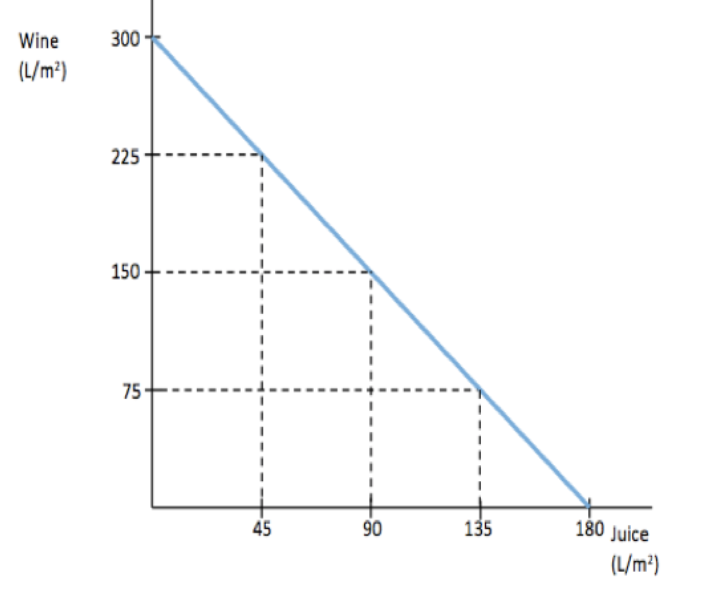
\includegraphics[width=0.6\linewidth]{cml_1_2_9}
\end{figure}
What is his opportunity cost of producing 1 litre of grape juice? Answer to the nearest two decimal places. [a] litres of wine.
\begin{align*}
	y &= 300 - \frac{75}{45}x\\
	&= 300 - \frac{75}{45}\\
	&= 298.33
\end{align*}
Therefore the opportunity cost is $300 - 298.33 = 1.67$

\subsection{Question 10}
Hilary owns a bakery and is trying to decide how to maximise her output. The two baked goods she sells are brownies and muffins. Shown below is Hilary's production possibilities curve. The X denotes the quantity of brownies and muffins she currently produces.
\begin{figure}[H]
	\centering
	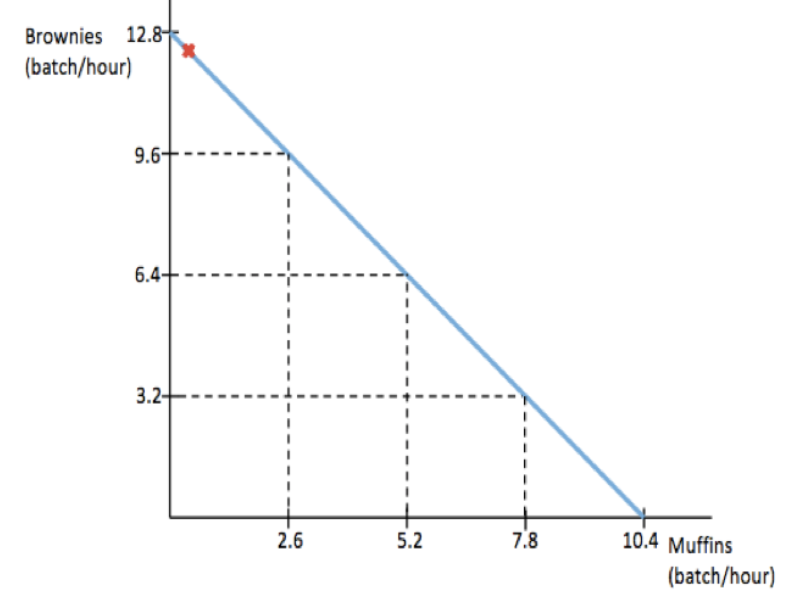
\includegraphics[width=0.6\linewidth]{cml_1_2_10}
\end{figure}
\noindent Is the current output attainable? (\hl{Yes}/No)\\
Is the current output \hl{efficient}, inefficient, or neither because it is unattainable?
Calculate the opportunity cost of producing 1 batch of muffins.
\begin{align*}
	y &= 12.8 - \frac{3.2}{2.6}x\\
	&= 12.8 - \frac{3.2}{2.6}\\
	&= 11.57
\end{align*}
Therefore the opportunity cost is $12.8 - 11.57 = 1.23$